\PassOptionsToPackage{unicode=true}{hyperref} % options for packages loaded elsewhere
\PassOptionsToPackage{hyphens}{url}
%
\documentclass[ignorenonframetext,]{beamer}
\usepackage{pgfpages}
\setbeamertemplate{caption}[numbered]
\setbeamertemplate{caption label separator}{: }
\setbeamercolor{caption name}{fg=normal text.fg}
\beamertemplatenavigationsymbolsempty
% Prevent slide breaks in the middle of a paragraph:
\widowpenalties 1 10000
\raggedbottom
\setbeamertemplate{part page}{
\centering
\begin{beamercolorbox}[sep=16pt,center]{part title}
  \usebeamerfont{part title}\insertpart\par
\end{beamercolorbox}
}
\setbeamertemplate{section page}{
\centering
\begin{beamercolorbox}[sep=12pt,center]{part title}
  \usebeamerfont{section title}\insertsection\par
\end{beamercolorbox}
}
\setbeamertemplate{subsection page}{
\centering
\begin{beamercolorbox}[sep=8pt,center]{part title}
  \usebeamerfont{subsection title}\insertsubsection\par
\end{beamercolorbox}
}
\AtBeginPart{
  \frame{\partpage}
}
\AtBeginSection{
  \ifbibliography
  \else
    \frame{\sectionpage}
  \fi
}
\AtBeginSubsection{
  \frame{\subsectionpage}
}
\usepackage{lmodern}
\usepackage{amssymb,amsmath}
\usepackage{ifxetex,ifluatex}
\usepackage{fixltx2e} % provides \textsubscript
\ifnum 0\ifxetex 1\fi\ifluatex 1\fi=0 % if pdftex
  \usepackage[T1]{fontenc}
  \usepackage[utf8]{inputenc}
  \usepackage{textcomp} % provides euro and other symbols
\else % if luatex or xelatex
  \usepackage{unicode-math}
  \defaultfontfeatures{Ligatures=TeX,Scale=MatchLowercase}
\fi
\usetheme[]{Copenhagen}
\usecolortheme{dolphin}
\usefonttheme{structurebold}
% use upquote if available, for straight quotes in verbatim environments
\IfFileExists{upquote.sty}{\usepackage{upquote}}{}
% use microtype if available
\IfFileExists{microtype.sty}{%
\usepackage[]{microtype}
\UseMicrotypeSet[protrusion]{basicmath} % disable protrusion for tt fonts
}{}
\IfFileExists{parskip.sty}{%
\usepackage{parskip}
}{% else
\setlength{\parindent}{0pt}
\setlength{\parskip}{6pt plus 2pt minus 1pt}
}
\usepackage{hyperref}
\hypersetup{
            pdftitle={Internship report at the Rwanda Revenue Authority},
            pdfauthor={Ogundepo Ezekiel Adebayo},
            pdfborder={0 0 0},
            breaklinks=true}
\urlstyle{same}  % don't use monospace font for urls
\newif\ifbibliography
\usepackage{color}
\usepackage{fancyvrb}
\newcommand{\VerbBar}{|}
\newcommand{\VERB}{\Verb[commandchars=\\\{\}]}
\DefineVerbatimEnvironment{Highlighting}{Verbatim}{commandchars=\\\{\}}
% Add ',fontsize=\small' for more characters per line
\usepackage{framed}
\definecolor{shadecolor}{RGB}{248,248,248}
\newenvironment{Shaded}{\begin{snugshade}}{\end{snugshade}}
\newcommand{\AlertTok}[1]{\textcolor[rgb]{0.94,0.16,0.16}{#1}}
\newcommand{\AnnotationTok}[1]{\textcolor[rgb]{0.56,0.35,0.01}{\textbf{\textit{#1}}}}
\newcommand{\AttributeTok}[1]{\textcolor[rgb]{0.77,0.63,0.00}{#1}}
\newcommand{\BaseNTok}[1]{\textcolor[rgb]{0.00,0.00,0.81}{#1}}
\newcommand{\BuiltInTok}[1]{#1}
\newcommand{\CharTok}[1]{\textcolor[rgb]{0.31,0.60,0.02}{#1}}
\newcommand{\CommentTok}[1]{\textcolor[rgb]{0.56,0.35,0.01}{\textit{#1}}}
\newcommand{\CommentVarTok}[1]{\textcolor[rgb]{0.56,0.35,0.01}{\textbf{\textit{#1}}}}
\newcommand{\ConstantTok}[1]{\textcolor[rgb]{0.00,0.00,0.00}{#1}}
\newcommand{\ControlFlowTok}[1]{\textcolor[rgb]{0.13,0.29,0.53}{\textbf{#1}}}
\newcommand{\DataTypeTok}[1]{\textcolor[rgb]{0.13,0.29,0.53}{#1}}
\newcommand{\DecValTok}[1]{\textcolor[rgb]{0.00,0.00,0.81}{#1}}
\newcommand{\DocumentationTok}[1]{\textcolor[rgb]{0.56,0.35,0.01}{\textbf{\textit{#1}}}}
\newcommand{\ErrorTok}[1]{\textcolor[rgb]{0.64,0.00,0.00}{\textbf{#1}}}
\newcommand{\ExtensionTok}[1]{#1}
\newcommand{\FloatTok}[1]{\textcolor[rgb]{0.00,0.00,0.81}{#1}}
\newcommand{\FunctionTok}[1]{\textcolor[rgb]{0.00,0.00,0.00}{#1}}
\newcommand{\ImportTok}[1]{#1}
\newcommand{\InformationTok}[1]{\textcolor[rgb]{0.56,0.35,0.01}{\textbf{\textit{#1}}}}
\newcommand{\KeywordTok}[1]{\textcolor[rgb]{0.13,0.29,0.53}{\textbf{#1}}}
\newcommand{\NormalTok}[1]{#1}
\newcommand{\OperatorTok}[1]{\textcolor[rgb]{0.81,0.36,0.00}{\textbf{#1}}}
\newcommand{\OtherTok}[1]{\textcolor[rgb]{0.56,0.35,0.01}{#1}}
\newcommand{\PreprocessorTok}[1]{\textcolor[rgb]{0.56,0.35,0.01}{\textit{#1}}}
\newcommand{\RegionMarkerTok}[1]{#1}
\newcommand{\SpecialCharTok}[1]{\textcolor[rgb]{0.00,0.00,0.00}{#1}}
\newcommand{\SpecialStringTok}[1]{\textcolor[rgb]{0.31,0.60,0.02}{#1}}
\newcommand{\StringTok}[1]{\textcolor[rgb]{0.31,0.60,0.02}{#1}}
\newcommand{\VariableTok}[1]{\textcolor[rgb]{0.00,0.00,0.00}{#1}}
\newcommand{\VerbatimStringTok}[1]{\textcolor[rgb]{0.31,0.60,0.02}{#1}}
\newcommand{\WarningTok}[1]{\textcolor[rgb]{0.56,0.35,0.01}{\textbf{\textit{#1}}}}
\usepackage{graphicx,grffile}
\makeatletter
\def\maxwidth{\ifdim\Gin@nat@width>\linewidth\linewidth\else\Gin@nat@width\fi}
\def\maxheight{\ifdim\Gin@nat@height>\textheight\textheight\else\Gin@nat@height\fi}
\makeatother
% Scale images if necessary, so that they will not overflow the page
% margins by default, and it is still possible to overwrite the defaults
% using explicit options in \includegraphics[width, height, ...]{}
\setkeys{Gin}{width=\maxwidth,height=\maxheight,keepaspectratio}
\setlength{\emergencystretch}{3em}  % prevent overfull lines
\providecommand{\tightlist}{%
  \setlength{\itemsep}{0pt}\setlength{\parskip}{0pt}}
\setcounter{secnumdepth}{0}

% set default figure placement to htbp
\makeatletter
\def\fps@figure{htbp}
\makeatother

\title{Internship report at Planning and Research department}
%\subtitle{Planning and Research department}
\author[The author]{
\includegraphics[height=5.6cm,width=9cm]{Images/Logo1.JPG}\\Ogundepo Ezekiel Adebayo}
\date{November 28, 2018}


\begin{document}
\frame{\titlepage}

\begin{frame}{}
\protect\hypertarget{section}{}

\begin{figure}
\centering
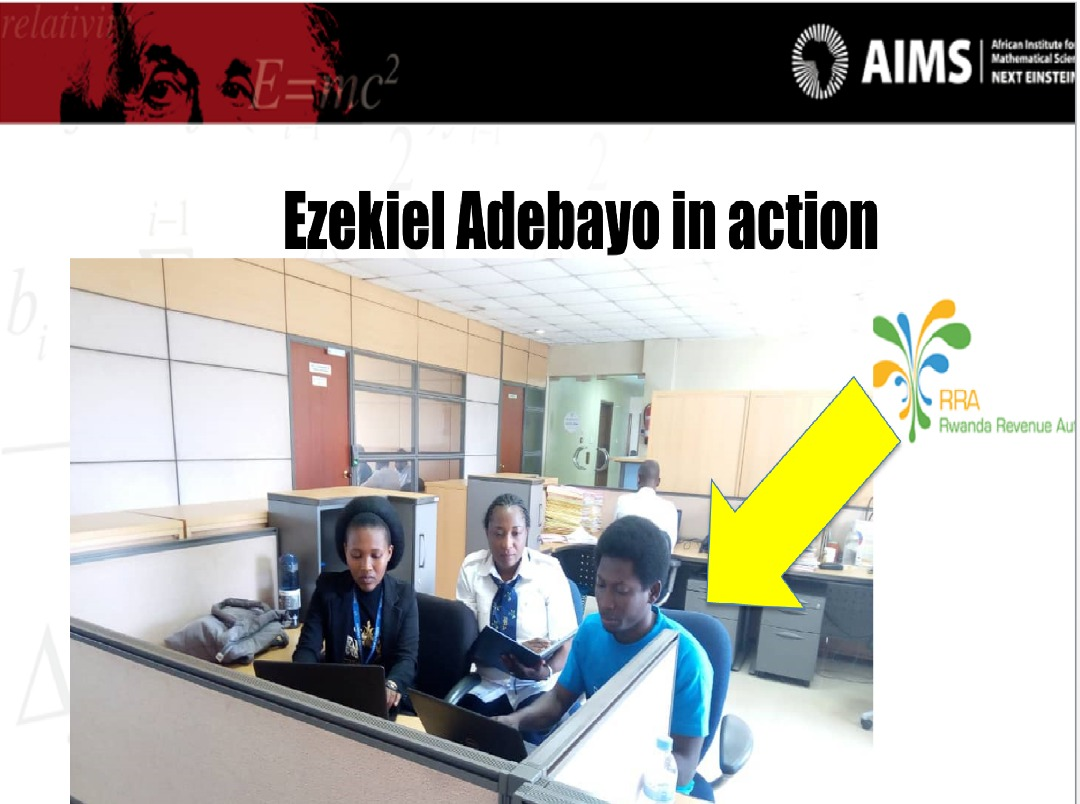
\includegraphics{Images/Ezekiel_in_action.jpeg}
\caption{Ezekiel in action}
\end{figure}

\end{frame}

\begin{frame}{Table of contents}
\protect\hypertarget{table-of-contents}{}

\begin{itemize}
\tightlist
\item
  AIMS/RRA Terms of References
\item
  On Job training
\item
  Managed and responded to various requests of data

  \begin{itemize}
  \tightlist
  \item
    Internal and External
  \end{itemize}
\item
  Give back to the community
\item
  Automations
\item
  Personal Professional Development at RRA
\end{itemize}

\end{frame}

\begin{frame}{Terms of Reference}
\protect\hypertarget{terms-of-reference}{}

As it is in the \textit{AIMS/RRA} terms of references, the AIMS interns
will contribute to various analyses done in Planning and Research
Department and automate some of the key analyses.

\end{frame}

\begin{frame}{}
\protect\hypertarget{section-1}{}

\begin{center}
\textbf{On Job training}
\end{center}

\end{frame}

\begin{frame}{On Job training}
\protect\hypertarget{on-job-training}{}

\begin{enumerate}
\tightlist
\item
  Insight with RRA domain. This included:

  \begin{enumerate}
  \tightlist
  \item
    Taxation theory
  \item
    BI and DWH
  \end{enumerate}
\item
  Insight on the various data that were used in the publication of
  \textit{Tax Statistics in Rwanda}.
\item
  Attended IMF training on models to estimate Tax expenditure for Rwanda
  : the training was held at Hotel des Milles Collines, from June 18 to
  June 22, 2018
\end{enumerate}

\end{frame}

\begin{frame}{}
\protect\hypertarget{section-2}{}

\begin{center}
\textbf{Managed and responded to various requests of data}
\end{center}

\end{frame}

\begin{frame}{Managed and responded to various requests of data}
\protect\hypertarget{managed-and-responded-to-various-requests-of-data}{}

\begin{enumerate}
\tightlist
\item
  Split sales annex \textit{big data} that were used by IMF team in the
  exercise of estimating VAT tax expenditure for Rwanda.
\end{enumerate}

\begin{block}{Summary of the file}

The file was more than 20 million rows, it was difficult to work with
that size with local processing software such as Excel, SPSS and Stata.
We used \textbf{\#Rstats} to do data wrangling by tidying the data,
split the data on a monthly and quarterly basis so that IMF would carry
further work on it.

\end{block}

\end{frame}

\begin{frame}{Managed and responded to various requests of data}
\protect\hypertarget{managed-and-responded-to-various-requests-of-data-1}{}

\begin{enumerate}
\setcounter{enumi}{1}
\tightlist
\item
  Contributed to data prepared for MINICOM with regards to the value of
  transactions made by firms registered in Made in Rwanda policy.
\end{enumerate}

The request was to do analysis based on \textbf{TIN},
\textbf{Business Income} and \textbf{Taxes}.

\end{frame}

\begin{frame}{Managed and responded to various requests of data}
\protect\hypertarget{managed-and-responded-to-various-requests-of-data-2}{}

\begin{enumerate}
[1)]
\setcounter{enumi}{2}
\tightlist
\item
  Quarterly payment of domestic taxes for Manufacturing Vs
  Non-manufacturing from 2007 to 2018\_Q1
\end{enumerate}

\begin{block}{Summary of the analysis}

Taxpayer's period years were classified according to quarters and tax
payment was classified according to manufacturing and non-manufacturing
companies using \textbf{ISIC} code.

\end{block}

\end{frame}

\begin{frame}{Managing and responding to various requests of data}
\protect\hypertarget{managing-and-responding-to-various-requests-of-data}{}

\begin{enumerate}
[1)]
\setcounter{enumi}{3}
\tightlist
\item
  Handling big data for VAT sales annexes
\end{enumerate}

Data wrangling was done for VAT sales annex data 2013-2017 by deleting
confidential information. The data were used by the researcher from
Harvard University working with IGC on the Consumer Incentives project
to evaluate the EBM lottery and potential rebate system.

\begin{block}{Structure of the file}

The VAT sales annexes data were Big data with more than 30 million rows
just for one fiscal year.

\end{block}

\end{frame}

\begin{frame}

\begin{center}
\textbf{Give back to the community}
\end{center}

\end{frame}

\begin{frame}{R for data science training class}
\protect\hypertarget{r-for-data-science-training-class}{}

\begin{figure}
\centering
\includegraphics{Images/training_1.jpg}
\caption{R for data science training}
\end{figure}

\end{frame}

\begin{frame}

Twelve (12) RRA staff followed the training for
\textit{\textbf{R for data science}} (R programming language). The
training was held in the offices of Planning and Research Department.

The staff came from Planning and Research Department, and Risk
Management Department, especially in the following units:

\begin{itemize}
\tightlist
\item
  Statistics Division (P \& RD)
\item
  Research Division (P \& RD)
\item
  Corporate Planning Division (P \& RD)
\item
  BI \& DWH unit (P \& RD)
\item
  IT\_Risk Management (RMD)
\end{itemize}

Also, 4 interns in Planning and Research Department attended the
training.

\end{frame}

\begin{frame}[fragile]{R codes demonstration}
\protect\hypertarget{r-codes-demonstration}{}

\begin{Shaded}
\begin{Highlighting}[]
\NormalTok{data <-}\StringTok{ }\KeywordTok{tribble}\NormalTok{(}
  \OperatorTok{~}\StringTok{`}\DataTypeTok{Unit(s)}\StringTok{`}\NormalTok{,}\OperatorTok{~}\StringTok{  `}\DataTypeTok{Number of attendees}\StringTok{`}\NormalTok{,}
\StringTok{'Statistics unit'}\NormalTok{, }\DecValTok{3}\NormalTok{,}
\StringTok{'Research unit'}\NormalTok{ , }\DecValTok{2}\NormalTok{,}
\StringTok{'Planning unit'}\NormalTok{ ,}\DecValTok{2}\NormalTok{,}
\StringTok{'IT_ Risk management unit'}\NormalTok{, }\DecValTok{2}\NormalTok{,}
\StringTok{'BI & DWH unit'}\NormalTok{,    }\DecValTok{2}\NormalTok{,}
\StringTok{'Interns in R&P, and RMD'}\NormalTok{, }\DecValTok{4}\NormalTok{,}
\StringTok{'ODI fellow'}\NormalTok{,}\DecValTok{1}\NormalTok{,}
\StringTok{'Total'}\NormalTok{,}\DecValTok{16}\NormalTok{)}
\end{Highlighting}
\end{Shaded}

\end{frame}

\begin{frame}{Output of R codes}
\protect\hypertarget{output-of-r-codes}{}

\begin{table}[ht]
\centering
\caption{List of participants in the R for data science training} 
\begin{tabular}{rlr}
  \hline
 & Unit(s) & Number of attendees \\ 
  \hline
1 & Statistics unit & 3 \\ 
  2 & Research unit & 2 \\ 
  3 & Planning unit & 2 \\ 
  4 & IT\_ Risk management unit & 2 \\ 
  5 & BI \& DWH unit & 2 \\ 
  6 & Interns in R\&P, and RMD & 4 \\ 
  7 & ODI fellow & 1 \\ 
  8 & Total & 16 \\ 
   \hline
\end{tabular}
\end{table}

\end{frame}

\begin{frame}{What we covered during R session training}
\protect\hypertarget{what-we-covered-during-r-session-training}{}

R programming language was introduced to the staff for the first time.
We covered some syntax that will prepare them for the use of R and make
their R programming enjoyable.

\begin{itemize}
\tightlist
\item
  Various atomic data types and structures
\item
  Data import to R and export from R.
\item
  R packages for data wrangling
\item
  Data manipulations and analysis
\item
  Data visualization
\end{itemize}

\end{frame}

\begin{frame}

\begin{figure}
\centering
\includegraphics{Images/training_2.jpg}
\caption{R for data science training}
\end{figure}

\end{frame}

\begin{frame}

\begin{center}
\textbf{Automation}
\end{center}

\end{frame}

\begin{frame}{Creation of data portal and automation of tax statistics}
\protect\hypertarget{creation-of-data-portal-and-automation-of-tax-statistics}{}

\begin{itemize}
\tightlist
\item
  Tax revenue by sector
\item
  Tax revenue by enterprise size
\item
  Tax revenue by enterprise type
\item
  Part A: Tax revenue by Enterprise type description
\item
  Part B: Tax revenue by Enterprise type description
\item
  Tax revenue by department
\end{itemize}

The portal is \href{https://bit.ly/taxrevenue}{here}

\end{frame}

\begin{frame}{Automation of VAT turnover}
\protect\hypertarget{automation-of-vat-turnover}{}

\begin{itemize}
\tightlist
\item
  VAT turnover by main sections of the economy
\item
  VAT turnover by main sectors of the economy
\end{itemize}

\end{frame}

\begin{frame}{Automation of Revenue Performance Analysis}
\protect\hypertarget{automation-of-revenue-performance-analysis}{}

\begin{itemize}
\tightlist
\item
  CIT and PIT
\item
  3\% WHT
\item
  5\% WHT
\item
  15\% WHT
\end{itemize}

\end{frame}

\begin{frame}{Professional Development at RRA}
\protect\hypertarget{professional-development-at-rra}{}

\begin{itemize}
\tightlist
\item
  Initiative and innovative
\item
  Problem solving
\item
  Power BI
\item
  Advanced R programming
\item
  ggplot2
\item
  SQL
\item
  ddplyr
\item
  Advanced Excel Training
\item
  Networking
\end{itemize}

\end{frame}

\begin{frame}{}
\protect\hypertarget{section-3}{}

\begin{center}
\textbf{Murakoze}
\end{center}

\end{frame}

\end{document}
